\documentclass[a4paper,12pt]{report}
\usepackage[utf8]{inputenc}
%\usepackage[frenchb]{babel}
\usepackage[T1]{fontenc}
\usepackage{lmodern,textcomp}
\usepackage{graphicx}
%\usepackage{listings}
\usepackage{caption}
%\usepackage{fancybox}
\usepackage[pdftex]{hyperref}
%\usepackage{epsfig}
\usepackage{fancyvrb}
\usepackage{tikz}
\usetikzlibrary{shapes.geometric,backgrounds,fit,positioning,trees}
\usetikzlibrary{shapes.callouts}
%\usetikzlibrary{arrows.meta,shapes.callouts}
\usepackage{wrapfig}
\usepackage{manfnt}
\usepackage{dingbat}
\usepackage{xcolor}
\usepackage{geometry}

\definecolor{reddebian}{rgb}{0.84314,0.03922,0.32549}
\definecolor{bluedane}{rgb}{0.09020,0.56863,1}
\definecolor{greendane}{rgb}{0.43137,0.60784,0.14510}
\def\purpledane{violet}

\hypersetup{%
  pdftitle={Xia},
  pdfauthor={Énuma Logiciel Libre},
  pdfsubject={Xia},
  pdfkeywords={Xia, logiciel libre, html5, Inkscape},
  colorlinks= true,
  linkcolor = greendane,
  urlcolor = bluedane
  }

% La dimension des marges
\geometry{hscale=0.7,vscale=0.7}

\title{Xia\\ Create HTML5 "images-actives"}

\renewcommand{\thechapter}{\arabic{chapter}}
\renewcommand{\thesection}{\Roman{section}}
\renewcommand{\thesubsection}{\alph{subsection}}

% pour unifier les indications relatives aux manipulation à effectuer dans les logiciels
% à modifier au besoin
\newcommand{\chemin}[1]{\texttt{\textcolor{reddebian}{#1}}}

% L'environnement alerte                        
\newsavebox{\boiteBrouillon}
\newcommand{\virageDanger}{\textdbend}

\newlength{\LargeurBouleAlerte}
\settowidth{\LargeurBouleAlerte}{%
  
\begin{tikzpicture}%
    \node{\virageDanger};%
  \end{tikzpicture}%
}

% Style pour la boîte alerte
\tikzstyle{boitealerte}=[draw=red,rounded corners,inner xsep=1em,inner ysep=1ex]

% Style pour la boule alerte
\tikzstyle{boulealerte}=[circle,ball color=red,text=white] 

\newenvironment{alerte}{%
  \begin{lrbox}{\boiteBrouillon}% On sauve dans \boiteBrouillon le contenu
    \begin{minipage}{.8\linewidth}%  
      \color{red}%
      \setlength{\parskip}{1ex plus 0.2ex minus 0.2ex}%
}{%
    \end{minipage}%
  \end{lrbox}% Fin. Attention lrbox stocke du contenu sur 1 ligne (pas de paragrpahe)
  % La boîte peut être utilisée via \usebox{\boiteBrouillon}
  \vspace{1.5ex}%
  
\begin{tikzpicture}%
    \node [boitealerte] (cadre) {%
      \hspace{0.5\LargeurBouleAlerte}%
      \usebox{\boiteBrouillon}%
    };%
    \node [boulealerte] (alerte) at (cadre.west) {\virageDanger};%
  \end{tikzpicture}%
  \vspace{1.5ex}%
}        

% L'environnement astuce
\newcommand{\pouceOK}{\large\leftthumbsup}

\newlength{\LargeurBouleAstuce}
\settowidth{\LargeurBouleAstuce}{%
  \begin{tikzpicture}%
    \node{\pouceOK};%
  \end{tikzpicture}%
}

\tikzstyle{bouleastuce}=[circle,ball color=teal,text=white]

\tikzstyle{boiteastuce}=[draw=teal,rounded corners,inner xsep=1em,inner ysep=1ex]
                        
\newenvironment{astuce}{%
  \begin{lrbox}{\boiteBrouillon}% On sauve dans \boiteBrouillon le contenu
    \begin{minipage}{.8\linewidth}%
      \color{teal}%
      \setlength{\parskip}{1ex plus 0.2ex minus 0.2ex}%
}{%
    \end{minipage}%
  \end{lrbox}% Fin. Attention lrbox stocke du contenu sur 1 ligne (pas de paragrpahe)
  % La boîte peut être utilisée via \usebox{\boiteBrouillon}
  \vspace{1.5ex}%
  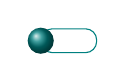
\begin{tikzpicture}%
    \node [boiteastuce] (cadre) {%
      \hspace{0.5\LargeurBouleAstuce}%
      \usebox{\boiteBrouillon}%
    };%
    \node [bouleastuce] (astuce) at (cadre.west) {\pouceOK};%
  \end{tikzpicture}%
  \vspace{1.5ex}%
}    

% L'environnement links
\newcommand{\mainDroite}{\large\leftpointright}

\newlength{\LargeurBouleLinks}
\settowidth{\LargeurBouleLinks}{%
  \begin{tikzpicture}%
    \node{\mainDroite};%
  \end{tikzpicture}%
}

\tikzstyle{boulelinks}=[circle,ball color=\purpledane,text=white]

\tikzstyle{boitelinks}=[draw=\purpledane,rounded corners,inner xsep=1em,inner ysep=1ex, align=right]
                        
\newenvironment{links}{%
  \begin{lrbox}{\boiteBrouillon}% On sauve dans \boiteBrouillon le contenu
    \begin{minipage}{.8\linewidth}%
      \color{\purpledane}%
      \setlength{\parskip}{1ex plus 0.2ex minus 0.2ex}%
}{%
    \end{minipage}%
  \end{lrbox}% Fin. Attention lrbox stocke du contenu sur 1 ligne (pas de paragrpahe)
  % La boîte peut être utilisée via \usebox{\boiteBrouillon}
  \vspace{1.5ex}%
  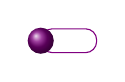
\begin{tikzpicture}%
    \node [boitelinks] (cadre) {%
      \hspace{0.5\LargeurBouleLinks}%
      \usebox{\boiteBrouillon}%
    };%
    \node [boulelinks] (links) at (cadre.west) {\mainDroite};%
  \end{tikzpicture}%
  \vspace{1.5ex}%
}    
\begin{document}
 
 \tableofcontents
 
 % il y a, à plusieurs reprises, des paragraphes du style "<à noter"> ou "<astuces">
 % peut-être faut-il adopter le style utilisé pour ce genre de choses dans la doc se3?
 
\section{Introducing Xia}

\subsection{What is Xia ?}

Xia is a free software developped by teachers of french academy of Versailles
It is released under "\\href{http://www.gnu.org/copyleft/gpl.html}{GPLv3} license.
Xia converter which takes as input a svg file and outputs an image-active in 
html5. Beyond the already known templates export user software ImagesActives 
(\\href{http://images-actives.crdp-versailles.fr/spip.php?article11&lang=fr}
{(accordion, buttons, etc.}), Xia further allows to generate
Interactive activities : games drag and drop, discrimination, selection, etc.

This document will help you «~step by step~» to create an image-active
Beginning with a simple image-active (crop, comments without particular 
enlightnings), it brings the user to a more complex image-active (multimedia
 enlightenments, games etc.). All examples are on line (each link is written at 
the beginning of the section), and svg source files are also available. At the end
on each part, a heading "Abstract" presents the essential guide lines to 
remember when creating an image-active.
\subsection{General process}

Unlike "ImagesActives", Xia is only needed at the end of the process.
As we can see on illustration \\ref{workflow_xia}, most of the work is done with 
a  vector graphics editor. We recommend to use the free open-source and 
muliplatform software \href{http://www.inkscape.org/}{Inkscape}, which is 
really easy to use (Inkscape will be used in this document).

\begin{figure}[htp]
 \centering
 \caption{Creation process of an image-active with  Xia}
 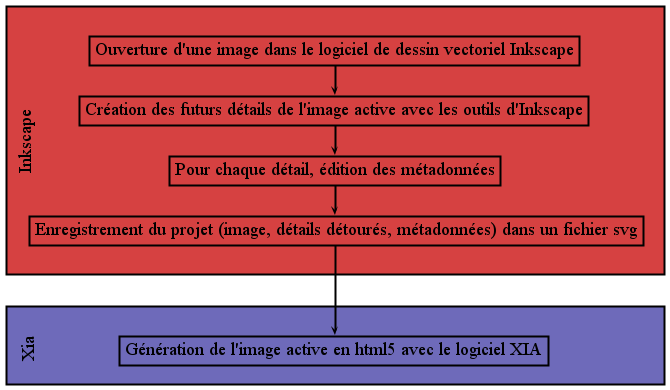
\includegraphics[width=1\textwidth]{images/workflow_xia}
 \label{workflow_xia}
\end{figure}

\section{Creating your first image-active using Inkscape and Xia: Basic features}

\subsection{Installing Inkscape and Xia}

Having Inkscape and Xia installed on your computer is the only thing you need 
to read this documentation.You will find any relevant informations about the 
installation of these softwares on their website :\\footnote{See the site 
\\href{http://www.inkscape.org/}{Inkscape} and \\href
{http://images-actives.crdp-versailles.fr/beta/}{Xia}.}.

\subsection{Building the svg source file to generate an image-active}\label{preparation_svg}

% cette phrase est répétée en début de chaque section: il faudrait trouver un moyen de la mettre en valeur
Explore the \\href{http://geoffrey-gekiere.ac-versailles.fr/xia1}{image-active 
created to illustrate this part of the document} and download the \\href
{http://geoffrey-gekiere.ac-versailles.fr/xia1/svg/xia1.svg}{svg source file}.

Manipulations described in this section will help you to
create a "basic" image-active featuring :
\begin{itemize}
 \item Zoom-in enabled details
 \item Details comments made only with raw text
\end{itemize}


Once you've chosen the image you will work with, open it with Inkscape 
(\\chemin{File} menu, then \\chemin{Open}).  When asked by the software
if you wish to «~\\chemin{Link or incorporate image}~», choose «~\\chemin
{Incorporate}.

Among the many details that one can learn by accessing the 
dialog window \\chemin{document} Metadata (\\chemin
{File} menu), three will be included in the image-active once
generated : title, creator, rights. They are therefore strongly.
recommended to inquire. In the following example (see figure \\ref
{titre_ia}), we see the importance of a title correctly entered in
Metadata: This is actually the title of the image-active  \\footnote {The
fields «~author~» and «~rights~» appear in the window
«~About~», symbolized by a clickable button shaped like the letter «~i~»}.

\begin{figure}[htp]
 \centering
 \caption{The title entered in the metadata of the document appears above 
the image-active and gives its name to the web page of it. The creator and 
 rights associated appear in the pop up associated with the «~i~» button 
on the right of the title of the image-active.}
 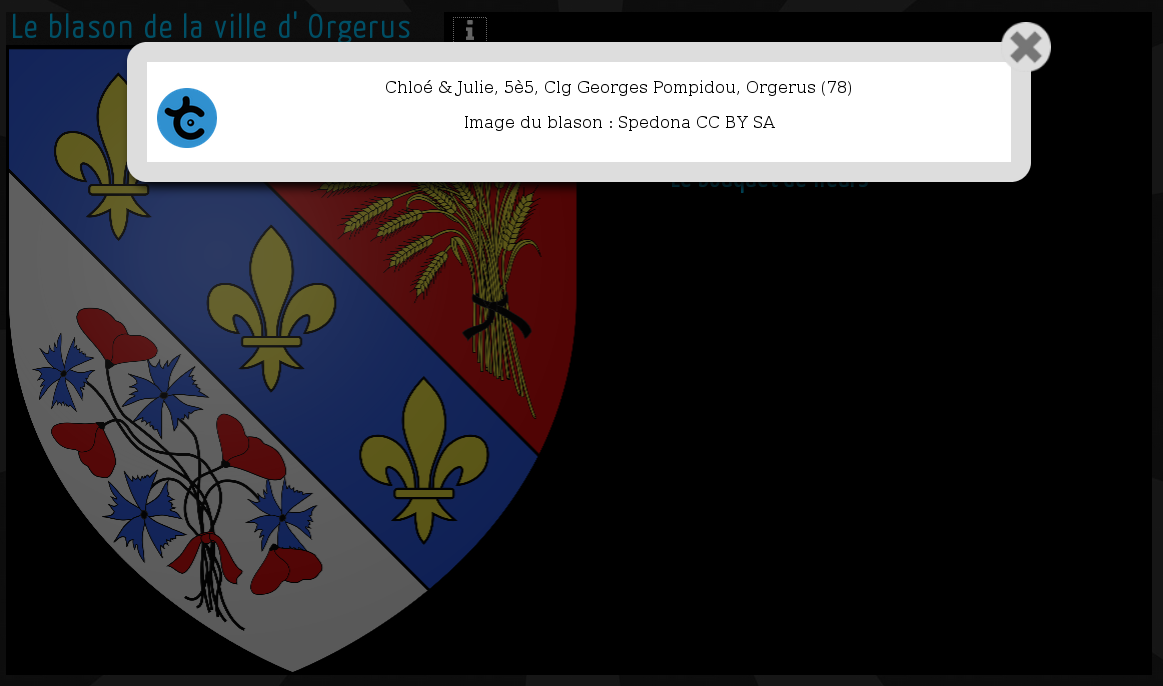
\includegraphics[width=\textwidth]{images/titre_ia}
 \label{titre_ia}
\end{figure}

We can save the image in svg format in the earlywork, 
through the way \chemin{File} menu, then \\chemin{Save as...}. 
For more clarity, we will remove the current extension of the image 
in the fields \chemin{Name) of the dialog window. Finally, in the 
dropdown dropdown menu, choose the Inkscape svg file format. \chemin{SVG Inkscape (*.svg)}.

Several Inkscape tools can be used to clip the details that
will become active in the animation generated by Xia . Among these :
\begin{itemize}
 \item 
\includegraphics[scale=0.5]{./images/rec_carre} Tool \chemin{Create rectangles and squares}
 \item 
\includegraphics[scale=0.5]{./images/cercles} Tool \chemin{Create circles, ellipses and arcs}
 \item 
\includegraphics[scale=0.5]{./images/lignes} Tool \chemin{Draw freehand lines}
 \item 
\includegraphics[scale=0.5]{./images/bezier} Tool \chemin{Bezier curves and straight lines}
\end{itemize}

% dans ce paragraphe, peut-être insérer une bidouille quelconque pour que l'allusion aux touches
% Ctrl et Maj soit plus claire (dessiner une touche de clavier?)
Without going in the detail of how these tools work\footnote{For this, 
refer to \href{http://inkscape.org/doc/shapes/tutorial-shapes.fr.
html}{Inkscape manual}.}, it will be noted that the «~\chemin
{Create rectangles and squares}~» and «~\\chemin{Create circles, 
ellipses and arcs}~»  tools can only be manipulated with the mouse or 
in relation with the keyboard :by pressing the Ctrl key, one draw a square, 
circle or rectangle of dimensions of integer (2: 1, 3: 1, etc.), and 
by pressing the Shift key, draw around the starting point.

The tool «~\chemin{Draw Bezier curves and straight lines}~» 
allows to crop «~click by click~» (work points are called 
«~nodes~»).  Figure is closed by clicking on the start node. 
The tool «~Bezier curves~» is called by keeping the mouse button pressed 
after creating a node, then moving the cursor to bring up the control handles 
to shape the curve segment as desired.

Note:
\begin{itemize}
 \item if the user sets in Inkscape a left open shape (for
example : a line), Xia will automatically close it  by connecting a 
 straight line between the beginning and the end of it.
 \item The order of creation of details in the image is generated in display 
order of the details (for example, detail first created in
Inkscape appears at the top in the image-active).)\footnote{if you wish to 
change that sequence without having to create the details once more, see 
section \ref{couche_XML}.}
\end{itemize}

Once a detail is cutted out, you can select it with the tool  
\chemin{Select and transform object} to resize it, to" 
move it, etc.

It is with a right click on the cut out detail that you access to 
\chemin{Object properties} (see illustration \ref{proprietes_objet}), and 
thus to the dialog window in which you add the text to be associated with the 
detail in the image-active.

\begin{figure}[htp]
 \centering
 \caption{The "Object properties" allows to enter the text that will become a 
 comment for the detail in the image-active}
 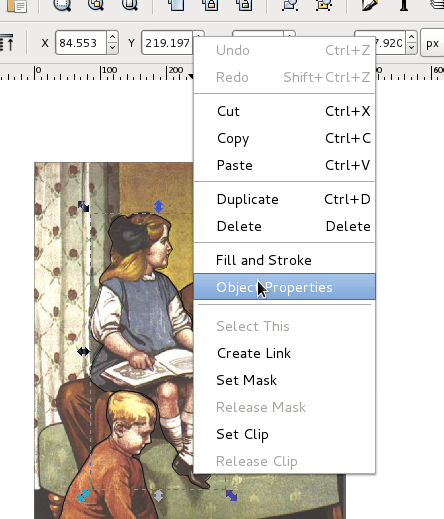
\includegraphics[width=0.5\textwidth]{./images/proprietes_objet}
 \label{proprietes_objet}
\end{figure}

The two fields to be filled in this window are \\chemin{Title} and 
\chemin{Description}.  The title filled in here will be the one of the detail, 
description will be its comment.

The process described above must also be done with the background image : 
the title and description indicated here will serve as an introduction to 
the image-active (title and comment not related to a particular detail).

\subsection{Generating the image-active with Xia}

\begin{figure}[htp]
 \centering
 \caption{Xia interface}
 
\includegraphics[width=0.8\textwidth]{./images/xia_vue_generale}
 \label{xia_interface}
\end{figure}

When all the details are clipped and their metadata indicated, one can launch 
Xia (see figure  \ref{xia_interface}). The first icon on the top left allows 
to select the svg source file.

\begin{center}

\includegraphics[scale=0.4]{./images/xia_open} 
\end{center}

Clicking on one of the icons export generates a series of files, including a 
\verb|index.html|. Warning : this file will not display anything if used 
alone. All the other files and directories generated during the export process 
must be stored in  the same folder as the \verb|index.html| file in order to 
the animation to work properly. \ textbf {It is therefore essential to 
dedicate a specific directory for each exported image}. Finally, just open 
the \verb| index.html| file in a web browser to see the image-active.

"Basic" Images actives templates are :
% pertinence d'ajouter une 4e colonne pour décrire brièvement les 
% caractéristiques de chaque export?
\begin{center}
\begin{tabular}{|c|c|p{3in}|}
\hline
Template name & Icon look & What you should know\\
\hline
\href{http://geoffrey-gekiere.ac-versailles.fr/xia1/accordionBlack}
{accordionBlack}  & 
\includegraphics[scale=0.5]{./images/accordionBlack} & 
Large comment zone, suitable for insertion of multimedia resources; to be used 
with vertical images (portrait)\\
\hline
\href{http://geoffrey-gekiere.ac-versailles.fr/xia1/accordionCloud}
{accordionCloud} &  
\includegraphics[scale=0.5]{./images/accordionCloud}& 
Narrow comment zone, with more space for the image itself ; to be used with 
horizontal images (landscape)\\
\hline
\href{http://geoffrey-gekiere.ac-versailles.fr/xia1/buttonBlue}{buttonBlue}&  

\includegraphics[scale=0.5]{./images/buttonBlue} & No lateral comment zone ; 
comments appear above the image (suitable for long comments) ; users access  
comments through icons placed above the image-active \\
\hline
\href{http://geoffrey-gekiere.ac-versailles.fr/xia1/popBlue}{popBlue} & 

\includegraphics[scale=0.5]{./images/popBlue} & No lateral comment zone; 
first click on the detail reveals it, and a second one pops up the comment 
(no zoom) \\
\hline
\href{http://geoffrey-gekiere.ac-versailles.fr/xia1/popYellow}{popYellow} & 

\includegraphics[scale=0.5]{./images/popYellow} & No lateral comment zone ; 
first click on the detail reveals it, and a second one simultaneously unveils 
the comment and the zoom function zoom sur le détail\\
\hline
\end{tabular}
\end{center}

\subsection{Abstract}

\begin{enumerate}
 \item An image-active is first build in Inkscape (svg format). Xia only 
 converts the svg source file into an html5 animation
 \item Title of the image-active must be indicated in the \chemin{Metadatas of 
the document}
 \item The text of the details is filled in the \chemin{Object properties}, 
 in the \chemin{Title} and \chemin{Description} fields
 \item General description of the image-active must be indicated in the \chemin
{Object properties} of the background image
\end{enumerate}

\section{Enriched image-active}

Explore the \href{http://geoffrey-gekiere.ac-versailles.fr/xia2}{image-active 
created for this section of the documentation} and download the 
\href{http://geoffrey-gekiere.ac-versailles.fr/xia2/svg/xia2.svg}{svg}.

In this section, the goal is still to create a "traditionna" image-active 
(ie. in which a detail matches a comment), but the content of the comments 
will be enriched with  formatted text or multimedia resources.

\subsection{Formatting text}

In ordre to insert formatted text, the following tags should be used :

% problème d'alignement du contenu des cellules sur les lignes "<liste de puces"> et "<tracer une ligne">
\begin{center}
 \begin{tabular}{|l|l|}
 \hline
  Tag & Result\\
  \hline
  \hline
  ***bold*** & \textbf{bold}\\
  \hline
  **italic** & \textit{italic}\\
  \hline
  [http://dane.ac-versailles.fr Le site de la Dane] & \href{http://dane.ac-versailles/fr}{Dane website}\\
  \hline
  \{\{\{Plain text\}\}\} & 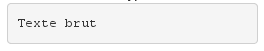
\includegraphics[scale=0.7]{./images/texte_brut}\\
  % là, faudrait symboliser les espaces simple et double pour les listes de puces
  \hline
  ~* a list\\
  ~* of bullets\\
  ~~* out of 2\\
  ~~* levels\\ & 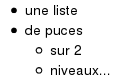
\includegraphics[scale=0.7]{./images/liste_puce}\\
  \hline
  drawing\\
  \verb|----|\\
  a line\\ & 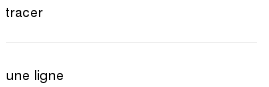
\includegraphics[scale=0.7]{./images/ligne_commentaire}\\
  \hline
  \end{tabular}
\end{center}

\subsection{Inserting multmedia resources into details}\label{enrichissement_multimedia}

Inserting multimedia resources into detail comments is quite easy: just paste 
the resource url (relative or absolute link) or iframe tag of the web service 
you want to use (for example, \href{https://scolawebtv.crdp-versailles.fr/}
Scolawebtv}).

Xia will automatically create a multimedia player in the comment as long as 
the resource (image, sound or video) matches its supported formats: 
\begin{description}
 \item [Images] jpg, jpeg, png, gif
 \item [Audio] ogg, mp3
 \item [Video] ogv, webm, mp4
\end{description}

The link is just inserted into the thread of comments to the detail:
\begin{description}
 \item[Absolute link] If the resource url is\\
 \begin{center}
 \verb|http://web.crdp.ac-versailles.fr/02546.ogg|\\
 \end{center}
 Just type that url inside description of the properties of the object in 
 Inkscape
 \item [Relative link] If the multimedia file is located in the image-active 
 folder or in a folder wihtin this one, just indicate its location, keeping in 
 mind that the image-active folder has to be considered as the root folder. 
 For example, if the \verb|video.ogv| file is located in a \verb|videos| 
 folder located itself in the image-active exportation folder, just indicate:\\
 \begin{center}
  \verb|videos/video.ogv|
 \end{center}
  in order to create the player
\end{description}

Since video formats supported by Xia are not natively supported by every web 
browsers, it is recommanded to export videos into the 3 supported formats, 
and to upload them into a single folder (from there, the only difference 
between those files is their extension (ie. .ogv or .mp4 or .webm):\\

% je pense qu'il y a moyen de faire vachement plus joli pour représenter l'arborescence
 % po4a: environment tikzpicture {} 
\begin{tikzpicture}
\end{tikzpicture}
 % po4a: environment alltt {} 
\parbox{0.40\textwidth}
{
\begin{alltt}
 -\textcolor{blue}{imageactive\_folder}\\
 ---index.html\\
 ---[files and folders generated by Xia]\\
 ---\textcolor{blue}{videos\_folder}\\
 -----video.mp4\\
 -----video.ogv\\
 -----video.webm\\
\end{alltt}
}
\fbox{\begin{minipage}{0.50\textwidth}
In this example, the folders (pointed out with blue type), were manually 
created by the image-active designer.  Folder \textcolor{blue}
{imageactive\_folder} contains the files et folders generated by Xia from the 
svg source file, including the index.html file. The \textcolor{blue}
{videos\_folder} was also manually created, in order to host videos inserted 
in the comments of the image-active using relative links.
      \end{minipage}}


Thus, even if a particular format is indicated in the description (following 
the previous example : \verb|repertoire_videos/video.ogv|), if the browser is 
unable to read the resource, it will automatically attempt to read the files 
of the same name possessing a different extension (ie. \verb|video.mp4| 
then \verb|video.webm|).

The last option is to insert in the commentary the iframe code hosting service 
resources. This will be interpreted and the reader will appear in the comment, 
giving access to the resource.

\subsection{The "audioBrown" template: sounds instead of text}

The "audioBrown" template is specifically dedicated to creation of 
images-actives in which details are associated with sounds rather than text.

The method to insert sounds using absolute or relative links is described in 
section \ref{enrichissement_multimedia}. If you wish the sound to play 
automatically as the user click on the comment, just add \verb|autostart|right 
after the url \footnote{The \\verb|autostart| tag also works with the other 
Xia templates.}:\\"
\begin{center}
 \verb|sons/son_detail_1.ogg autostart|
\end{center}


\subsection{Inserting images into your image-active}\label{insertion_images}

Png images can be added to the background image-active. To do this, in 
Inkscape, go in the \\chemin{File} menu, and choose \chemin{Import} 
to incorporate your new image.

Imported image will only appear in image-active if applied white background in 
Inkscape (choose white in the horizontal colour palette at the bottom of 
Inkscape interface (see illustration \ref{remplissage_blanc}).

\begin{figure}[htp]
 \centering
 \caption{In Inkscape, select the embedded png then apply a white background 
 by selecting the color from the horizontal colour palette to make it 
 automatically visible} 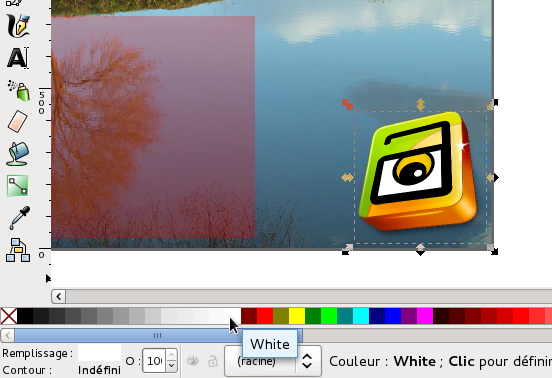
\includegraphics[width=0.6\textwidth]
 {images/remplissage_blanc}
 \label{remplissage_blanc}
\end{figure}

By indicating a URL in the \chemin{Title} of \chemin{Object properties} field, 
the embedded image becomes a clickable icon linking to a web page.

\subsection{Displaying a question and unveiling an answer}

Designer can create an "\textit{Answer}" clickable icon, momentarily 
preventing user to read the end of the comment.

To do so, just indicate, in the description, the line\\ \verb|Answer:| or 
\verb|answer:| followed by the text you wish to be showed.

\subsection{Controlling details behavior : automatic display and disabled zoom}
\label{couche_XML}

Default behavior of details in an image-active consists in:
\begin{itemize}
 \item highlighting details only on mouse over or with a click on the comment 
 detail title
 \item zoom in effect when clicking again on the active detail\footnote{Except 
 for the popBlue template.}
\end{itemize}

Both of these default behaviors can be modified if the designer applies a white
 or black background to cropped details (see section \ref{insertion_images} 
 and illustration \ref{remplissage_blanc):
\begin{description}
 \item [Detail whith a white background] Dans l'image générée, 
 le détail sera immédiatement visible, sous la forme d'un aplat de couleur opaque (masquant
 logiquement l'image de fond), qui une fois sélectionné, révêle l'image de fond (le détail demeure zoomable)
 \item [Détail auquel est appliqué un fond de couleur noire] Le détail n'est visible qu'en étant sélectionné, mais
 n'est pas zoomable.
\end{description}

Conséquence logique: un détail ne pouvant se voir appliquer à la fois un fond blanc et noir, il ne peut être à la
fois immédiatement visible \textit{et} non-zoomable.

\subsection{Contrôler l'ordre d'affichage des détails dans l'image active}

Par défaut, dans l'image active générée, les détails apparaissent verticalement dans l'ordre 
dans lequel les détails correspondants ont été créés (le premier détail créé dans Inkscape 
correspondant au détail placé en haut dans la barre latérale de l'image active).

On passera par l'\chemin{Éditeur XML} dans le menu \chemin{Édition} pour modifier cet 
ordre par défaut.

A priori complexe à gérer, cette fenêtre de dialogue se laisse en réalité apprivoiser aisément: 
la sélection sur l'image des détails met en évidence les entrées XML correspondantes, qu'il n'y 
a donc plus qu'à les glisser-déposer à l'endroit désiré (voir figure \ref{ordre_couches}).

De ce fait, l'utilisateur qui modifie fréquemment l'ordre de ses détails devrait prendre l'habitude 
de renseigner pour chacun d'eux le champs \chemin{ID} de ses propriétés, afin d'être en mesure 
de le manipuler plus aisément dans l'\chemin{Éditeur XML}.

\begin{figure}[htp]
 \centering
 \caption{L'éditeur XML d'Inkscape permettant de contrôler l'ordre d'affichage des détails dans l'image 
 active générée. On remarquera la mise en évidence d'un élément dans l'éditeur et sur l'image de fond 
 par simple clic de souris.}
 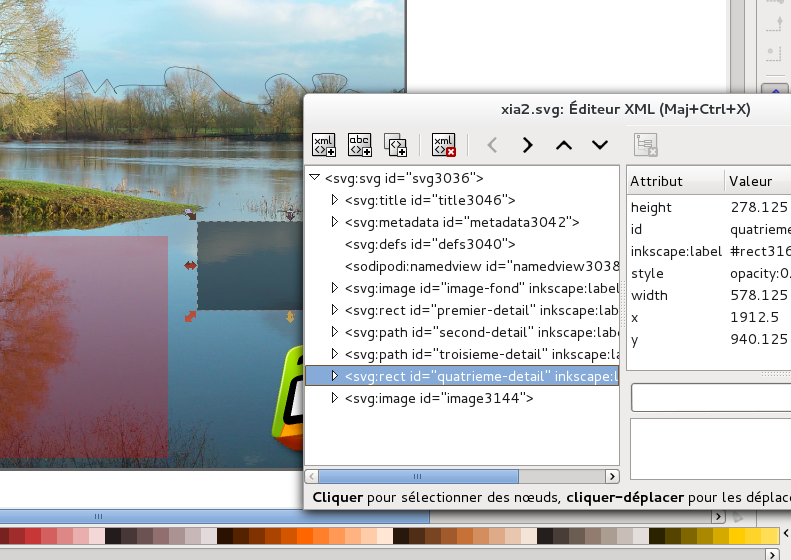
\includegraphics[width=\textwidth]{images/ordre_couches}
 \label{ordre_couches}
\end{figure}

\subsection{Pour résumer}

\begin{enumerate}
 \item On peut enrichir et mettre en forme le texte en utilisant des balises
 \item Un enrichissement multimédia est possible par un simple lien relatif ou absolu vers un fichier 
 dont le format est reconnu par Xia
 \item L'ajout d'images sur l'image de fond est possible par simple importation de celles-ci
 \item On modifie le comportement par défaut d'un détail en changeant sa couleur de fond (blanc, noir)
 \item L'ordre des détails dans l'image active générée dépend de l'ordre de création de ceux-ci, 
 mais reste modifiable via l'éditeur XML d'Inkscape
\end{enumerate}


\section{De l'interactivité à l'activité: réaliser des jeux avec Xia}

Jusqu'à présent, cette documentation a uniquement abordé la réalisation d'images actives au sens «~traditionnel~»:
une image de fond dont des détails détourés sont associés à des commentaires plus ou moins enrichis.

Ce type d'image permet de mettre en œuvre des scénarios pédagogiques ne manquant pas d'intérêt 
(découverte progressive de documents, fabrication par les élèves d'images actives), 
mais Xia va beaucoup plus loin en permettant la réalisation de jeux et d'activités variées, dans lesquelles
l'utilisateur est amené à réaliser infiniment plus d'actions que la simple lecture
 de commentaires...

\subsection{Premier principe ludique: sélectionner, retrouver dans l'image}

Explorez l'\href{http://geoffrey-gekiere.ac-versailles.fr/xia3}{image active créée pour cette section de la documentation} 
et téléchargez le \href{http://geoffrey-gekiere.ac-versailles.fr/xia3/svg/xia3.svg}{svg}.

\textit{Le principe ludique est le suivant: on propose une image dans laquelle l'utilisateur 
doit sélectionner un certain nombre de détails en fonction d'une consigne. 
La réalisation de l'objectif énoncé déclenche l'affichage d'un message.}

C'est en réalité l'activité, voire l'image active la plus simple à réaliser. Il suffit en effet 
au créateur de la ressource de détourer les éléments que l'utilisateur doit retrouver.

La consigne à destination de l'utilisateur de l'image active est à renseigner 
dans les métadonnées du document. En effet, au moment de l'export, Xia cherche les informations
situées dans le champs \chemin{Description} des métadonnées du document 
(voir section \ref{preparation_svg} et figure \ref{titre_ia}), afin d'en faire une «~pop up~»
qui s'affichera lors de l'ouverture de l'image générée. L'utilisateur lit alors la consigne et ferme
la pop up pour jouer.

Lorsque l'utilisateur a réussi le jeu, un message apparaît. 
Celui-ci est créé dans la \chemin{Description} des \chemin{Propriétés de l'objet} de l'image de fond
\footnote{Quand une image active «~traditionnelle~» est générée, cette manipulation
permet la création du commentaire introductif à l'image, non relié à un détail particulier
(voir section \ref{preparation_svg}).}. 
Deux informations sont nécessaires pour que ce message apparaisse:
le nombre de bonnes réponses déclenchant le message\footnote{Ce nombre est à la discrétion
du créateur de la ressource et peut tout à fait être inférieur au nombre total de détails placés sur l'image},
et le message en lui-même. Ce tableau résume les balises à insérer:

% le multicolumn refuse le \verb... à corriger
\begin{center}
 \begin{tabular}{|l|p{2in}|p{2in}|}
 % \hline
% \multicolumn{3}{|c|}{Informations à renseigner dans le champs Description des Propriétés de l'objet}\\
 \hline
  Objectif & Renseigner le nombre de bonnes réponses nécessaires pour terminer le jeu & Afficher un message\\
  \hline
  Balise & \verb|<score></score>| & \verb|<message></message>|\\
  \hline
  Exemple & \multicolumn{2}{|l|}{<score>6</score>}\\
   & \multicolumn{2}{|l|}{<message>Bravo, vous avez réussi à sélectionner}\\
    & \multicolumn{2}{|l|}{correctement tous les éléments demandés</message>}\\
  \hline
 \end{tabular}
\end{center}

Astuce: le texte inséré dans la balise \verb|<message></message>| peut 
tout à fait être enrichi. 
On peut ainsi imaginer de proposer le visionnage d'une image, d'une vidéo, ou l'affichage d'un lien vers un second exercice, afin 
de «~chaîner~» les activités par degré de difficultés.

La génération d'une l'image active ayant pour principe ludique la sélection de détails
correspond dans Xia à l'export \chemin{game1clic}:

\begin{center}

\includegraphics[scale=0.7]{./images/game1clic} 
\end{center}

\subsubsection{Pour aller plus loin... Comment montrer à l'utilisateur sa progression lors de l'utilisation d'un jeu game1clic?}\label{detail_progression}

On peut programmer l'apparition d'éléments visuels lorsque l'utilisateur sélectionne une réponse correcte. 
Ces éléments peuvent être issus de l'importation d'images au format png, mais également 
être directement créées dans Inkscape.
Cependant, puisque Xia considère comme un détail clicable tout élément créé à partir des outils 
d'Inkscape, il faudra, après avoir dessiné ceux-ci, les transformer en «~copie bitmap~».
Par exemple:
\begin{enumerate}
 \item On dessine une étoile de côtés jaune sur fond jaune avec les outils d'Inkscape
 \item Après avoir sélectionné cette étoile, on clique, dans le menu \chemin{Édition}, sur 
 \chemin{Faire une copie bitmap}
 \item On supprime l'étoile ayant servi à créer cette copie bitmap, devenue inutile
\end{enumerate}

Une fois les éléments visuels importés (fichiers png) ou créés (copie bitmap de figures créées à la main),
il suffit d'appliquer à ceux-ci la caractéristique
\begin{center}
\chemin{Interactivité > OnClick} = \verb|off|
\end{center}
et enfin de grouper le détail clicable à cet élément (en cliquant successivement sur le détail et l'élément visuel en maintenant 
la touche Maj enfoncée, puis en sélectionnant \chemin{Grouper} dans le menu \chemin{Objet} d'Inkscape).

\subsubsection{Pour aller plus loin... Comment mettre en évidence les erreurs de l'utilisateur dans un jeu game1clic?}

Le principe ludique de la sélection d'un ensemble de détails dans une image a un intérêt pédagogique évident... 
et des limites qui le sont tout autant (on imagine aisément un élève tenter de cliquer frénétiquement sur chaque pixel 
de l'image active sans réfléchir une seule seconde...).

C'est la raison pour laquelle il peut être intéressant d'être en mesure de mettre en évidence dans le jeu les erreurs commises 
par les utilisateurs.

Pour cela, le créateur de la ressource prévoiera de déposer aux endroits stratégiques de son image de fond, dans Inkscape, 
un élément visuel assez explicite pour symboliser l'erreur. Cet élément visuel peut être une 
image au format png ou une forme créée directement avec les outils de dessins d'Inkscape, puis transformée en bitmap 
(voir la méthode décrite à la section \ref{detail_progression}). 
On appliquera à celui-ci la caractéristique
\begin{center}
\chemin{Interactivité > OnClick} = \verb|disable-score| 
\end{center}
De cette manière, le détail demeure
clicable, mais son activation n'ajoute pas un point au compteur permettant au final de déclencher 
le message de victoire.

\subsection{Second principe ludique: classer, légender, hiérarchiser}

\textit{Second principe ludique: une image de fond contient des étiquettes qu'il faut déplacer et 
déposer sur les bons détails. Lorsque tous les éléments ont été remis à leur place, un message 
confirme la résolution du jeu.}

Explorez l'\href{http://geoffrey-gekiere.ac-versailles.fr/xia5}{image active créée pour cette section de la documentation} \\
et téléchargez le \href{http://geoffrey-gekiere.ac-versailles.fr/xia5/svg/xia5.svg}{svg}.

La démarche pour la réalisation d'un jeu de ce type est la suivante:
\begin{enumerate}
 \item Dans Inkscape:
\begin{itemize}
 \item Choisir une image de fond
 \item Préparer les «~étiquettes~» à déplacer (petites images ou texte)
 \item Faire correspondre chaque étiquette à sa zone de dépôt (en réalité, un détail détouré)
 grâce aux métadonnées renseignées
\end{itemize}
 \item Dans Xia
 \begin{itemize}
  \item Exporter le svg ainsi préparé avec le thème «~gameDragAndDrop~»
 \end{itemize}
\end{enumerate}

Deux méthodes sont envisageables pour disposer des «~étiquettes~» à déplacer.
Un moyen simple est d'utiliser un utilitaire de capture d'écran 
capable de produire des images au format png puis d'importer celles-ci dans Inkscape.
On peut également produire des étiquettes de type texte directement dans Inkscape en regroupant un 
cadre (outil \chemin{Créer des rectangles et des carrés}) et un élément textuel puis en 
faisant une copie bitmap de cet ensemble (voir section \ref{detail_progression})\footnote{... sans oublier, après avoir
fait la copie bitmap, de supprimer le regroupement devenu inutile.}.
On fait ensuite correspondre aux détails censés les accueillir\footnote{\textbf{Une} étiquette ne pouvant correspondre qu'à \textbf{un} détail.}.

Le tableau suivant résume les métadonnées à renseigner dans les \chemin{Propriétés de l'objet}
dans l'étiquette et le détail correspondant afin de les «~jumeler~»:

\begin{center}
\begin{tabular}{|p{1.in}|p{2.5in}|p{1.5in}|}
\hline
 & Étiquette (objet à déplacer) & Détail détouré (réceptacle de l'étiquette)\\
\hline
Champs ID & & \verb|Titre_Detail|\\
\hline
Champs Description & \verb|<target>Titre_Detail</target>| & \\
\hline
Champs Interactivité > Onclick & & \verb|off|\\
\hline
\end{tabular}
\end{center}

Pour résumer, le créateur de la ressource fait savoir à Xia quelle étiquette correspond à quel détail en faisant 
correspondre le champs \chemin{ID} du détail (réceptacle) au champs \chemin{Description} de l'étiquette 
(objet à déplacer). La seule subtilité consiste à entourer, dans le champs \chemin{Description}
de l'étiquette, l'ID correspondante d'une balise \verb|<target></target>|.

Une astuce: si l'image active contient de nombreux détails réceptacles de taille identique, 
on peut en créer une, lui appliquer la caractéristique \chemin{Interactivité > OnClick} = \verb|off|, 
puis copier-coller ce détail autant de fois que nécessaire. Conservant cette option, 
le créateur de la ressource n'aura pas besoin d'aller l'appliquer à chaque détail créé, 
et aura uniquement à modifier les champs \chemin{ID}.

La génération d'une l'image active ayant pour principe ludique le glisser déposer 
correspond dans Xia à l'export \chemin{gameDragAndDrop}:

\begin{center}

\includegraphics[scale=0.7]{./images/gameDragAndDrop} 
\end{center}

\subsubsection{Comment ajouter un effet «~magnétisme~» dans le jeu gameDragAndDrop}

En indiquant\\
\begin{center}
\verb|<magnet>on</magnet>| 
\end{center}
dans le champs \chemin{Description}
du détail réceptacle de l'étiquette, un effet «~aimant~» sera effectif au moment où 
l'utilisateur approche son étiquette de la cible.

L'avantage de cette option est qu'elle permet à l'utilisateur d'être sûr que 
la non-résolution du jeu provient d'une erreur de correspondance de ses 
étiquettes, et pas d'un léger décalage entre l'étiquette et la zone de dépôt.

\subsection{Pour résumer}

Aperçu synthétique des principales balises à insérer dans le cadre de
la création d'un jeu (export game1clic ou gameDragAndDrop):

\begin{center}
 \begin{tabular}{|p{1.5in}|p{1in}|p{1in}|p{1in}|p{1in}|}
 Balise & Quel rôle? & Sur quel objet? & À insérer dans... & Qu'y insérer?\\
 \hline
 \verb|<score></score>| & Indiquer le nombre de bonnes réponses déclenchant le message de fin & Image de fond & Propriétés de l'objet > Description & Le chiffre correspondant au score demandé\\
 \hline
 \verb|<message></message>| & Afficher le message de fin du jeu & Image de fond & Propriétés de l'objet > Description & Un message personnalisé, si besoin enrichi\\
 \hline
 \verb|off| & Rendre insensible au clic un détail & Détail & Propriétés de l'objet > Interactivité > Onclick & \\
 \hline
 \verb|disable-score| & Conserve la sensibilité au clic mais n'ajoute pas de point au compteur de résultat quand sélectionné & Détail & Propriétés de l'objet > Interactivité > Onclick & \\
 \hline
 \verb|<target></target>| & Indique au détail déplaçable son détail fixe correspondant & Détail à déplacer & Propriétés de l'objet > Description & Faire correspondre au champs ID de la cible\\
 \hline
 \verb|<magnet>on</magnet>| & Ajoute un effet «~aimant~» & Détail réceptacle & Propriétés de l'objet > Description & \\
 \end{tabular}
\end{center}


\end{document}
